\documentclass[11pt, a4paper]{article}

% ---- compact layout for a 1-2 page supervisor summary ----
\usepackage[T1]{fontenc}
\usepackage[utf8]{inputenc}
\usepackage{lmodern}
\usepackage[a4paper, margin=2.0cm, top=2.2cm, bottom=2.2cm]{geometry}
\usepackage{microtype}
\usepackage{amsmath, amssymb}
\usepackage{booktabs}
\usepackage{multirow}
\usepackage{array}
\usepackage{enumitem}
\usepackage{xcolor}
\usepackage{titlesec}
\usepackage{pgfplots}
\pgfplotsset{compat=1.18}
\usepackage[hidelinks]{hyperref}
\usepackage{setspace}

\definecolor{colSiamese}{HTML}{2166AC}
\definecolor{colArcFace}{HTML}{D6604D}
\definecolor{colAdaFace}{HTML}{4DAC26}
\definecolor{colGreen}{HTML}{66C2A5}
\definecolor{colRandom}{HTML}{FC8D62}
\definecolor{colOriginal}{HTML}{8DA0CB}
\definecolor{highlight}{HTML}{FFF3CD}
\definecolor{headerbg}{HTML}{EEF2F7}

\titleformat{\section}{\normalsize\bfseries\color{colSiamese}}{\thesection}{0.6em}{}[{\color{colSiamese}\titlerule[0.6pt]}]
\titlespacing{\section}{0pt}{1.2ex plus 0.3ex}{0.5ex plus 0.1ex}

\titleformat{\subsection}{\small\bfseries}{\thesubsection}{0.5em}{}
\titlespacing{\subsection}{0pt}{0.8ex}{0.2ex}

\setlength{\parskip}{0.3ex}
\setlength{\parindent}{0pt}

\newcommand{\good}[1]{\textcolor{colSiamese}{\textbf{#1}}}
\newcommand{\bad}[1]{\textcolor{colArcFace}{#1}}
\newcommand{\bestval}[1]{\textbf{#1}}

% =========================================================
\begin{document}

% ---- Title block ----------------------------------------
\begin{center}
  {\large\bfseries Open-Set Bat Face Recognition: Progress Report}\\[0.5em]
  {\small Sagi Levi \quad \texttt{lesagi@gmail.com} \quad June 2026}
\end{center}
\vspace{-0.3em}
\noindent\color{colSiamese}\rule{\linewidth}{1pt}\color{black}
\vspace{0.4em}

% ---- Summary paragraph ----------------------------------
\textbf{Goal.} Build a non-invasive system that identifies individual fruit bats from
facial images, supporting long-term behavioural studies without physical tagging.
The system handles \emph{open-set} scenarios: bats seen at test time were never
observed during training.

\textbf{Current status.} A three-model comparison (Siamese pair network, ArcFace,
AdaFace) has been completed across two species (rousettus, mauritius) and three
background conditions, using a rigorous identity-disjoint evaluation protocol.
A fully automated training and reporting pipeline is operational.

% ==========================================================
\section{Key Finding: Evaluation Protocol Matters}

A common pitfall in animal re-identification is \emph{identity leakage}: splitting
images randomly instead of splitting identities means the same bat appears in both
training and test sets, inflating results.
Table~\ref{tab:leakage} demonstrates the scale of this effect.

\begin{table}[h]
\centering
\caption{Same model, same data --- different splitting protocol.}
\label{tab:leakage}
\setlength{\tabcolsep}{8pt}
\begin{tabular}{lcc@{\hspace{6pt}}c}
\toprule
Protocol & ROC-AUC & F\textsubscript{1} & Recall \\
\midrule
Random-pair split \bad{(leaky)}          & 0.982 & 0.987 & 0.986 \\
\good{Identity-disjoint split (correct)} & 0.858 & 0.707 & 0.734 \\
\bottomrule
\end{tabular}
\end{table}

\textbf{Takeaway:} all results in this report use identity-disjoint splits exclusively.

% ==========================================================
\section{Model Comparison}

\subsection{Rousettus --- 12 individuals, 1\,059 images (6/3/3 id split)}

\begin{table}[h]
\centering
\caption{Test-set results on rousettus by background, 3 unseen test identities.
Siamese ROC-AUC is pairwise-head; ArcFace/AdaFace ROC-AUC is cosine-based (not directly
comparable). $^{\dagger}$ = not significant ($p<0.05$, permutation $n{=}100$).}
\label{tab:rousettus}
\setlength{\tabcolsep}{5pt}
\begin{tabular}{llccccc}
\toprule
Model & BG & ROC-AUC & F\textsubscript{1} & Top-1 & mAP & TAR@\(10^{-3}\) \\
\midrule
\good{Siamese}  & random & 0.858 & 0.707 & ---   & ---   & 0.012 \\
\good{Siamese}  & green  & 0.669 & 0.797 & ---   & ---   & 0.001 \\
ArcFace (v2)    & random & 0.665$^{\dagger}$ & --- & 0.532 & 0.731 & 0.074 \\
ArcFace (v2)    & green  & 0.847 & --- & \bestval{0.846} & \bestval{0.915} & 0.067 \\
AdaFace         & random & 0.434$^{\dagger}$ & --- & 0.274 & 0.560 & 0.003 \\
AdaFace         & green  & 0.753 & --- & 0.556 & 0.762 & 0.006 \\
ArcFace (v1)    & random & \bad{0.500}$^{\dagger}$ & --- & 0.591 & 0.757 & 0.000 \\
\bottomrule
\end{tabular}
\end{table}

\vspace{-0.2em}
\textbf{Note on ArcFace default:} paper-scale hyperparameters (SGD $\eta{=}0.1$,
margin $0.5$, scale $64$) destroy the ImageNet pretrained backbone --- validation
ROC-AUC stays at chance even as train accuracy climbs to $0.93$. Tuning to
Adam $\eta{=}10^{-3}$, margin $0.2$, scale $30$ recovers strongly on \emph{green}
backgrounds (ROC-AUC $0.847$, Top-1 $0.846$) but remains near chance on random
compositing --- a background effect, not a fixed identity-count ceiling.

\subsection{Mauritius --- 11 individuals, 1\,119 images (5/3/3 id split)}

\begin{table}[h]
\centering
\caption{Test-set results on mauritius across background conditions.
Siamese ROC-AUC is pairwise-head; ArcFace/AdaFace ROC-AUC is cosine-based.
$^{\dagger}$ = not significant ($p<0.05$).}
\label{tab:mauritius}
\setlength{\tabcolsep}{5pt}
\begin{tabular}{llccccc}
\toprule
Model & Background & ROC-AUC & F\textsubscript{1} & Top-1 & mAP & TAR@\(10^{-3}\) \\
\midrule
\good{Siamese} & green    & 0.710 & 0.689 & --- & ---   & 0.014 \\
\good{Siamese} & original & 0.834 & 0.753 & --- & ---   & 0.005 \\
\good{Siamese} & random   & 0.806 & 0.686 & --- & ---   & 0.007 \\
ArcFace        & green    & 0.843 & --- & 0.740 & 0.870 & 0.282 \\
AdaFace        & green    & \bestval{0.902} & --- & \bestval{0.916} & \bestval{0.955} & 0.383 \\
ArcFace        & original & 0.791 & --- & 0.576 & 0.774 & 0.145 \\
AdaFace        & original & 0.731 & --- & 0.634 & 0.785 & 0.151 \\
ArcFace        & random   & 0.578$^{\dagger}$ & --- & 0.479 & 0.697 & 0.021 \\
AdaFace        & random   & 0.539 & --- & 0.459 & 0.682 & 0.006 \\
\bottomrule
\end{tabular}
\end{table}

% ==========================================================
\section{ROC-AUC Summary (bar chart)}

\begin{center}
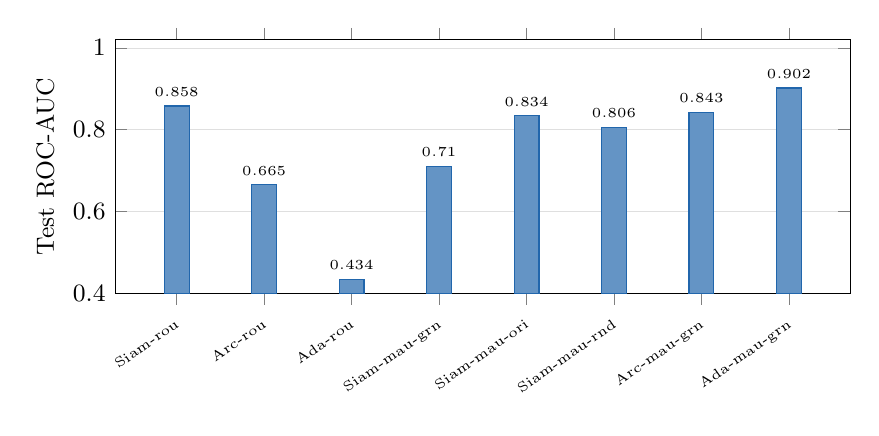
\begin{tikzpicture}
\begin{axis}[
  ybar, bar width=9pt,
  height=4.8cm, width=0.90\linewidth,
  ymin=0.4, ymax=1.02,
  ymajorgrids=true,
  grid style={line width=0.3pt, draw=gray!25},
  ylabel={Test ROC-AUC},
  symbolic x coords={
    Siam-rou,
    Arc-rou,
    Ada-rou,
    Siam-mau-grn,
    Siam-mau-ori,
    Siam-mau-rnd,
    Arc-mau-grn,
    Ada-mau-grn},
  xtick=data,
  xticklabel style={font=\tiny, rotate=35, anchor=north east},
  tick label style={font=\small},
  label style={font=\small},
  nodes near coords,
  nodes near coords align={vertical},
  nodes near coords style={font=\tiny,
    /pgf/number format/fixed,
    /pgf/number format/precision=3},
  legend style={font=\tiny, draw=none,
    at={(0.02,0.98)}, anchor=north west}
]
\addplot[fill=colSiamese!70, draw=colSiamese]
  coordinates {
    (Siam-rou,     0.858)
    (Arc-rou,      0.665)
    (Ada-rou,      0.434)
    (Siam-mau-grn, 0.710)
    (Siam-mau-ori, 0.834)
    (Siam-mau-rnd, 0.806)
    (Arc-mau-grn,  0.843)
    (Ada-mau-grn,  0.902)
  };
\end{axis}
\end{tikzpicture}
\end{center}

{\footnotesize
\textbf{x-axis key:}
Siam = Siamese, Arc = ArcFace, Ada = AdaFace;
rou = rousettus (random bg); mau = mauritius with grn/ori/rnd background.
Siamese bars are pairwise-head ROC-AUC, embedding bars cosine ROC-AUC (not directly
comparable; read within-family).
}

% ==========================================================
\section{Why Background --- Not Identity Count --- Drives the Gap}

After correcting the AdaFace margin, ImageNet normalisation, and evaluation resolution,
the embedding models are competitive at $\le\!13$ identities; what separates success from
collapse is the \textbf{background}, not the number of training identities.

\smallskip
\textbf{1.\ The train/test gap is background-dependent.}
Train accuracy is near-perfect in every condition, so identity count cannot explain the
gap; the background can.  With identity count fixed (6 train ids), the gap shrinks
sharply from random to green:

\begin{center}
\setlength{\tabcolsep}{6pt}
\begin{tabular}{llccc}
\toprule
Model & BG & Train acc & Test ROC-AUC & Gap \\
\midrule
ArcFace & random & 0.969 & 0.665 & $-0.304$ \\
AdaFace & random & 0.975 & 0.434 & $-0.541$ \\
ArcFace & green  & 0.998 & 0.847 & $-0.151$ \\
AdaFace & green  & 0.998 & 0.753 & $-0.245$ \\
\bottomrule
\end{tabular}
\end{center}

\smallskip
\textbf{2.\ Top-1 is at chance only on random backgrounds.}
With 3 unseen test identities, chance is 0.33.  On random backgrounds ArcFace/AdaFace
hover near it (rousettus 0.53/0.27); on green screen they soar (rousettus ArcFace 0.85,
mauritius AdaFace 0.92).  Transferable structure \emph{does} emerge when the background
is coherent.

\smallskip
\textbf{3.\ Instability tracks the background.}
ArcFace and AdaFace validation curves oscillate and (for AdaFace) decay on random
backgrounds, but converge to high, stable values on green/original --- the instability is
a property of the random-background landscape, not of the small class count.

\smallskip
\textbf{4.\ Cross-species consistency points to background.}
The pattern replicates for both species, ruling out species-specific causes:

\begin{center}
\setlength{\tabcolsep}{6pt}
\begin{tabular}{lccc}
\toprule
Species & ArcFace random & ArcFace green & $\Delta$ \\
\midrule
rousettus & 0.665 & 0.847 & $+0.182$ \\
mauritius & 0.578 & 0.843 & $+0.265$ \\
\bottomrule
\end{tabular}
\end{center}

Both species are weak on random compositing and both recover on green screen at the same
small identity counts, isolating \textbf{background coherence} as the governing variable.
Identity count likely still matters at larger scales, but it is not the binding constraint
we can demonstrate here.


\end{document}
